%!TEX root = ChapSpringer_Main.tex
\subsection{3D integration technology}
3D integration technology is considered to be one of the most promising paths to enable further scaling of Integrated Circuits (ICs). Over the past years many different 3D integration technology flavors have been proposed in both academia and industry. Depending on the integration granularity, a very coarse grain 3D technology classification differentiates between 3D-Stacked Integrated Circuits (3D-SICs) and 3D Monolithic integration. Each of these technology options has it's own merits and drawbacks and as of today there is no clear preference for one or the other. The right choice is very much design dependent and is strongly affected by our ability to perform optimal design implementation.

3D-SICs are built using 2 (or more) fully processed integrated circuits (wafers) that are integrated vertically one on the top of each other (i.e. dies are stacked). Different 3D structures that enable this particular type of 3D integration have been proposed over the past years and they typically include: wire bonding, Through Silicon Vias (TSV), micro-bumps and copper pads. Even if the wire bonding technique is well known, practical usage remained limited because of the connection pitch that is quite high (\~100 micrometer range). Also, wire bonds have high resistance and capacitance that will strongly affect delay and power of a 3D wire. Further, as wire bonds appear at the periphery of the IC, the signals connected to them need to be routed throughout the whole circuit. For all these reasons it is generally considered that the wire bonding is not well suited for efficient 3D integration. 

On the other hand TSVs, micro-bumps and copper pads are much more promising technology features since they can be manufactured at very low pitch, the diameter depends on the structure but is generally in the um range allowing dense 3D integration (many inter-die nets). These 3D structures also have good resistance and capacitance values, allowing small delay and power overheads of 3D nets compared to wire bonding and even 2D as long as we enable some wirelength savings for 3D. 

With these structures 3D circuits can be stacked in many different ways depending on the orientation of the circuit \emph{face}, i.e. the side of the IC where we find the active layer (transistors i.e. gates). Not all of the options are interesting from the integration perspective, Face-to-Face (F2F) and Face-to-Back (F2B) integration schemes are the ones that are used most of the time. Cross-sections of F2F and F2B 3D integration schemes is shown on Figure~\ref{fig:3D-Stacking}).

\begin{figure}[!b]%
\centering
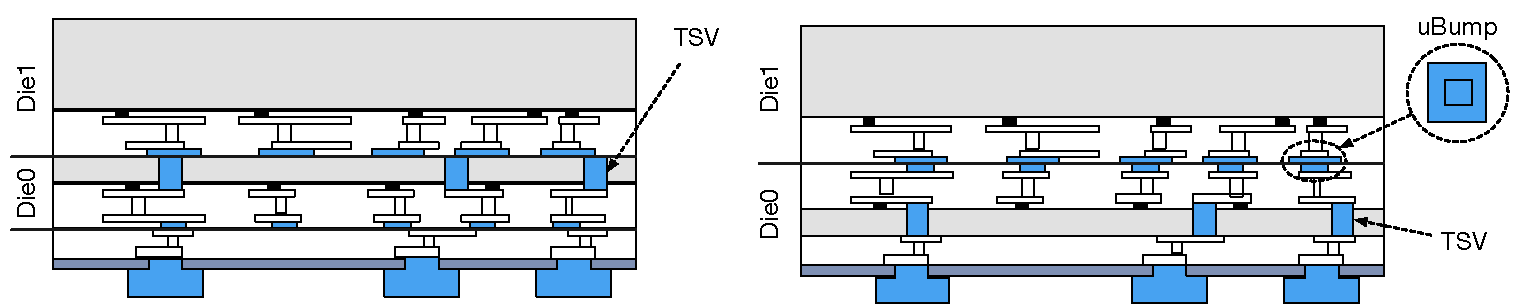
\includegraphics[width=0.95\columnwidth]{3D_IC.pdf}
\caption{Cross section of Face-to-Back and Face to Face 3D-Stacked Integrated Circuit\label{fig:3D-Stacking}}
\end{figure}

In F2F 3D-SIC, the face of both dies are oriented towards each other and they are interconnected directly. Input/output TSVs are used to connect the active layer of one of the dies to the package ensuring the system communication with the external world. F2F is in principal limited to stacking of two dies only (although it would be possible to stack yet another die on the top of the stack using F2B approach). In case of F2B 3D-SIC, face of one die is oriented towards the back of other die. The active layers of the dies are connected using TSVs, a vertical connection that goes through the substrate of the die. Active layer of one of the dies is exposed to the package used for communication of the system with the external world. F2B can be used to stack more than two dies and is used for manufacturing of highly dense SRAM and DRAM circuits.

The assembly of the dies can be carried out at die or at the wafer level, hence we distinguish: a) Die-to-Die, b) Die-to-Wafer, or c) Wafer-to-Wafer 3D integration. Each assembly method has its advantages (and disadvantages) and the choice depends on the application needs to realize the cost benefits of the 3D integration (trade-off between the wafer processing speed, yield and die area). From the design perspective, there is no significant difference in the choice of assembly approach. We can thus safely assume any of the proposed assembly methods. 3D stacking technology is mature today and is already used in production lines (e.g. DRAM/FLASH memories).

In 3D monolithic integration multiple transistor or logic gate layers are formed sequentially starting from the bottom-most layer. Minimal interconnect structures are used in between these layers: Monolithic Inter-Layer vias (MIVs) for vertical connections and very limited metal layers for horizontal connectivity. The dimension and parasitics of MIVs are of the order of a local via (in the range of nm). As a result, ultra fine-grained vertical integration of devices is possible. The integration grain is finer from the one of the 3D-SICs, since we can stack at lower level (transistor and gate). 

If the stacking is happening at the gate-level, the appropriate EDA tools should perform system partitioning at gate-level, and they should be able to place \& route the design in 3D. Note that current EDA tools are not ready for this, since the IC design was a 2D problem until today. If stacking happens at transistor level, the existing EDA, 2D, tools can be used because the problem is now moved to the one of the 3D standard cell design.  

While 3D monolithic integration is very promising, there are lot of issues that remain associated with the efficient wafer manufacturing. 3D monolithic process requires high-temperature operations that heavily impact the device performance. Thus, it is known that two consecutive layers will not have the same performance; the top layer having worse performance than the bottom layer, since it is processed afterwards. This will have important consequences on system design and will lower the benefits of such integration.

In the context of this work we focus on 3D-SIC circuits approach.